\section{引言}

\begin{figure}[t]
    \centering
    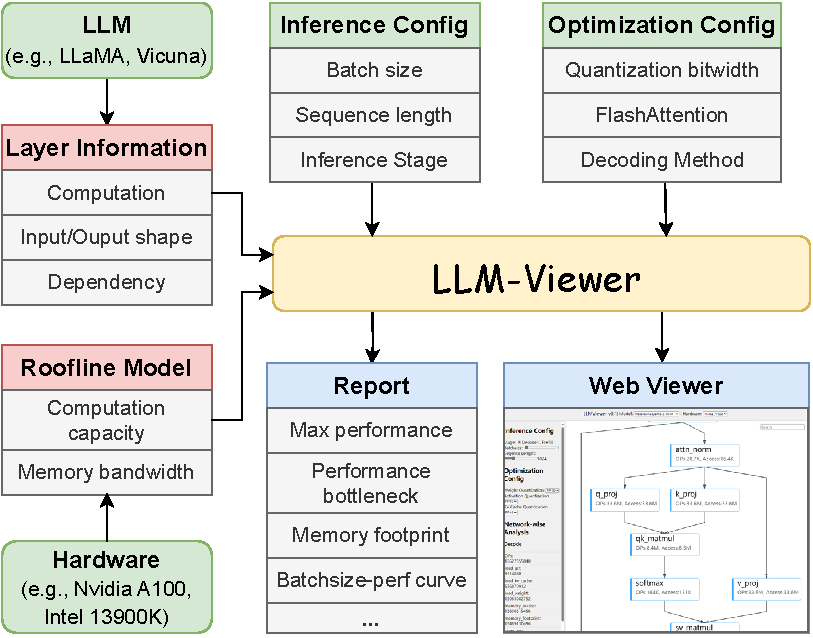
\includegraphics[width=0.95\linewidth]{ims/viewer_flowchat.pdf}
    \caption{\textbf{我们设计的 LLM-Viewer 工作流。}输入包括目标 LLM 部署配置与硬件设备信息。接收输入后，LLM-Viewer 会精确分析给定 LLM 在指定硬件上的部署瓶颈，并支持有针对性的高效推理优化。}
    \vspace{-0.2in}
    \label{fig:llmviewer_workflow}
\end{figure}

\begin{figure*}[t]
    \centering
    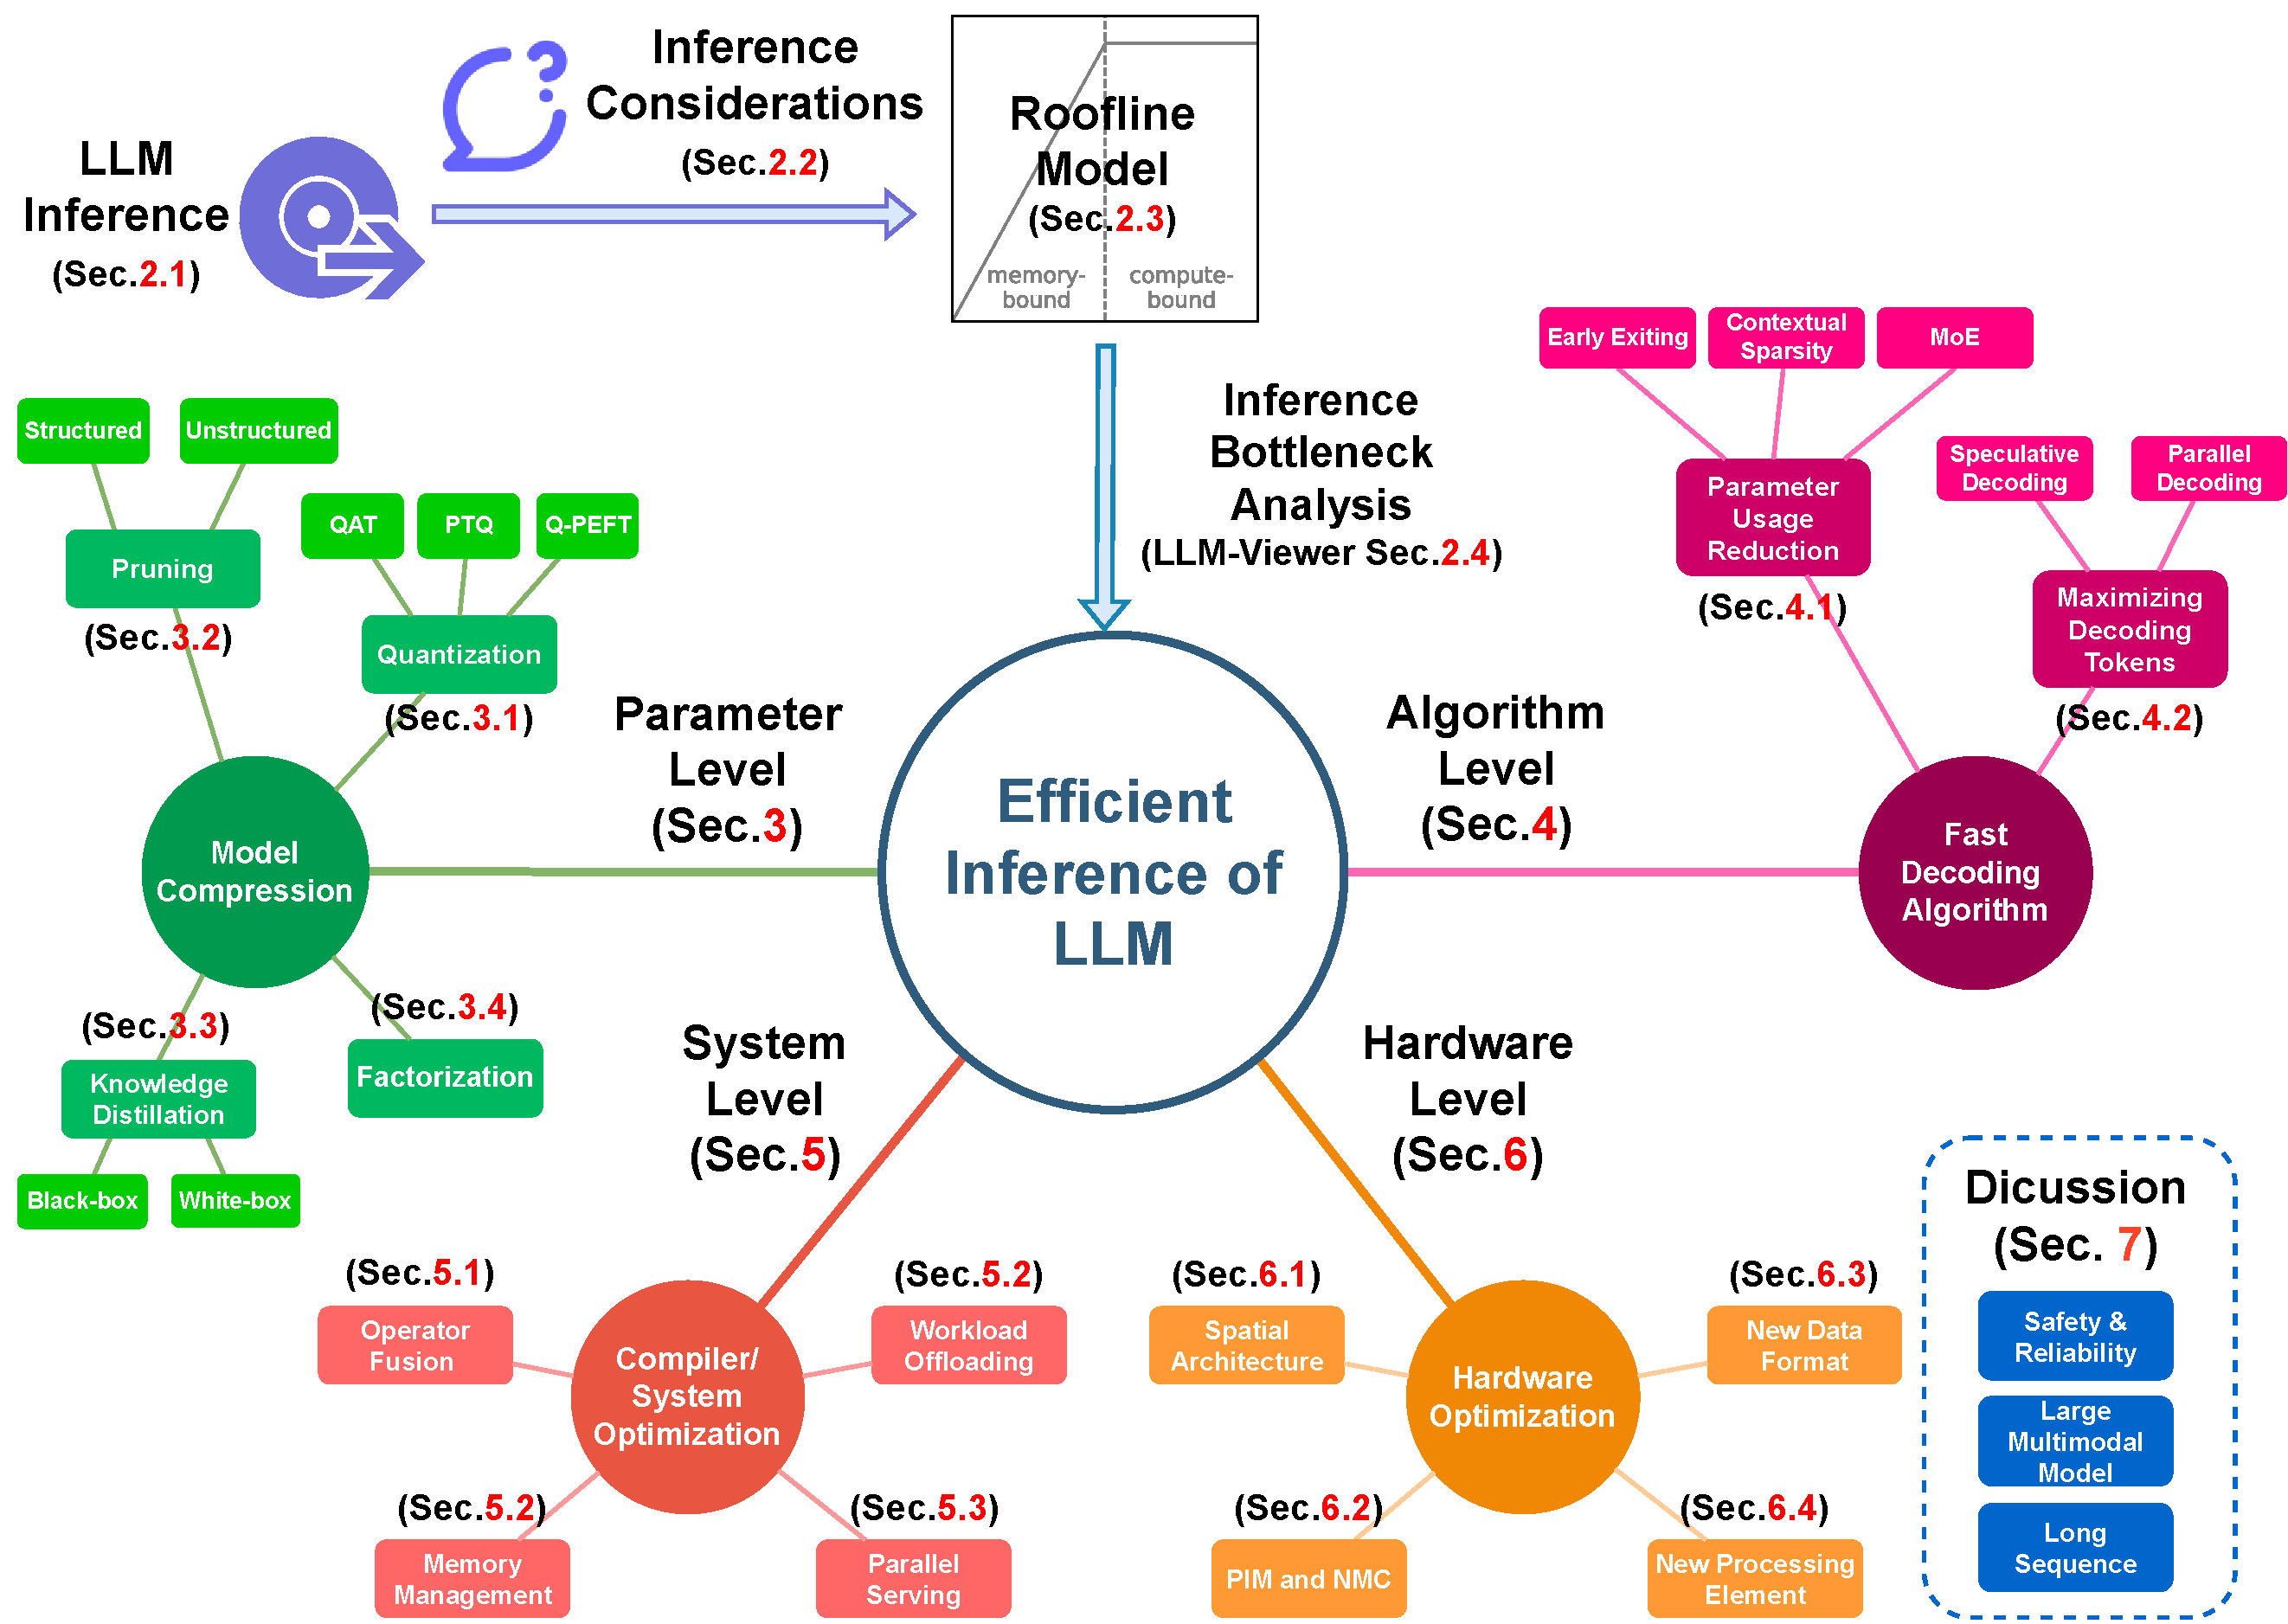
\includegraphics[width=0.96\textwidth]{ims/mindmap3.pdf}
    \caption{\textbf{高效 LLM 推理综述思维导图。}本综述不同于传统综述，重点关注 LLM 推理的工程实践问题。我们首先识别并分析 LLM 推理挑战，然后引入定制化 Roofline 模型定位瓶颈（Sec.\ref{sec:challenges}）。随后将推理效率优化分为四个方向：参数压缩（Sec.\ref{sec:compression}）、快速解码算法（Sec.\ref{sec:fast-decoding}）、系统级优化（Sec.\ref{sec:system_optimization}）与硬件级优化（Sec.\ref{sec:hardware-optimization}）。}
    \vspace{-0.2in}
    \label{fig:mindmap}
\end{figure*}

近年来，大语言模型（LLM）已成为 AI 发展的核心力量，持续重塑机器学习与自然语言处理（NLP）格局~\citep{zhao2023survey}。
这一趋势可追溯到 ChatGPT~\citep{brown2020language,ouyang2022training} 等里程碑模型的成功，它们凭借强大的理解与生成能力产出高度拟人化文本。
随后，OPT~\citep{zhang2022opt}、BLOOM~\citep{scao2022bloom}、Llama~\citep{touvron2023llama1,touvron2023llama2} 等模型不断涌现，进一步强化了“更大模型通常具备更强能力”的共识。
因此，数十亿乃至数百亿参数模型已日益常见。

但模型规模的急剧增长也带来了严峻推理挑战。
这些挑战不仅影响算力受限设备，也同样影响最先进硬件平台。
由于模型复杂度高、规模大、能耗与计算成本高，LLM 在真实场景部署难度很大。
同时，高资源消耗还引发了能效、可扩展性与可及性的担忧，尤其对中小组织与计算资源有限社区更为不利。
因此，亟需创新方案使 LLM 推理更加普惠与可持续。

为解决部署难题，大量方法被提出。过去两年，高效 LLM 推理研究呈指数增长，机遇与挑战并存。
虽然研究繁荣，但信息量激增也可能掩盖关键趋势、拖慢进一步进展。
现有文献的关键缺口在于：缺乏统一、系统且面向实践的分析框架，以支撑跨方法对比与综合方案设计。

针对这一缺口，本文给出了高效 LLM 推理的全景综述，并强调实践驱动特征。
与传统综述不同，我们不仅归纳已有工作，还提出专门构建的 Roofline 分析模型，用于定位 LLM 部署瓶颈（图~\ref{fig:llmviewer_workflow}）。
据我们所知，这是首批面向“LLM 在硬件上的推理复杂性分析”提供工具化支撑的工作之一。
我们系统整理了最新进展，并围绕部署挑战（特别是推理效率）展开深入讨论，覆盖模型压缩、解码算法改进、系统优化与硬件优化（图~\ref{fig:mindmap}）。

同时，近期已有相关综述，例如 \citep{zhu2023survey} 关注 LLM 压缩，\citep{miao2023towards}、\citep{ding2023efficiency}、\citep{wang2024model} 关注整体服务系统。
而我们的差异化在于引入 Roofline 统一分析视角，从而更清晰连接算法机制与部署瓶颈。

本文结构如下：首先介绍 LLM 基础并给出工具 LLM-Viewer（Sec.\ref{sec:challenges}），该工具可基于 Roofline 模型分析任意 LLM 架构在不同硬件平台上的部署瓶颈（图~\ref{fig:llmviewer_workflow}）。
随后，本文将高效推理方法归纳为四类：模型压缩（Sec.\ref{sec:compression}）、快速解码算法（Sec.\ref{sec:fast-decoding}）、编译器/系统级优化（Sec.\ref{sec:system_optimization}）以及硬件级优化（Sec.\ref{sec:hardware-optimization}）。
